%Version 3.1 December 2024
% Manuscript for Computing (Springer Nature)

\documentclass[pdflatex,sn-mathphys-num]{sn-jnl}

\usepackage[T1]{fontenc}%
\usepackage[utf8]{inputenc}%
\usepackage{microtype}%
\usepackage{graphicx}%
\usepackage{multirow}%
\usepackage{amsmath,amssymb,amsfonts}%
\usepackage{booktabs}%
\usepackage{xcolor}%

\raggedbottom

\begin{document}

\title[A Comparative Study of Classical Lightweight ML for Text Classification]{A Comparative Study of Classical Lightweight Machine Learning Models for Text Classification}

\author*[1]{\fnm{Chaitanya} \sur{Mokkapati}}\email{chaitumokkapati@gmail.com}

\author[2]{\spfx{Dr.} \fnm{Prasad} \sur{Devarasetty}}

\author[1]{\fnm{Nagulmeera} \sur{Syyed}}

\affil*[1]{\orgdiv{Department of Artificial Intelligence and Machine Learning}, \orgname{DVR \& Dr.\ HS MIC College of Technology}, \orgaddress{\city{Kanchikacherla}, \state{Andhra Pradesh}, \country{India}}}

\affil[2]{\orgdiv{Department of Computer Science and Engineering}, \orgname{DVR \& Dr.\ HS MIC College of Technology}, \orgaddress{\city{Kanchikacherla}, \state{Andhra Pradesh}, \country{India}}}

\abstract{Text classification supports critical applications including spam filtering, news categorization, and content moderation. Although transformer-based models achieve high accuracy, their training and deployment frequently depend on GPU infrastructure, long runtimes, and substantial memory budgets that are often unavailable in academic and industrial settings with limited compute. This study investigates whether classical lightweight machine learning models can provide a practical alternative under strict CPU-only constraints. We benchmark five algorithms (Logistic Regression, Linear Support Vector Machine, Multinomial Naive Bayes, Random Forest, and XGBoost) using a unified TF-IDF feature pipeline on the SMS Spam Collection and AG News datasets. Beyond standard classification metrics, we report training time, inference latency, and serialized model size to quantify accuracy-efficiency trade-offs. Linear SVM achieves the highest F1-score of 94.1\% on SMS Spam and Logistic Regression achieves 90.2\% macro F1 on AG News, while Linear SVM delivers the lowest mean inference latency of 0.02~ms per 1{,}000 samples. The complete five-model benchmark finishes in approximately 2.6 minutes on a 2-core CPU. Wilcoxon tests show that differences among top-ranked models are not statistically significant at $\alpha=0.05$ with three repeated runs. The findings indicate that carefully selected classical models remain competitive for resource-constrained text classification and can be reproduced without GPU acceleration.}

\keywords{Text classification, Lightweight machine learning, TF-IDF, Comparative benchmarking, Computational efficiency, CPU-based deployment}

\maketitle

\section{Introduction}\label{sec:introduction}

Text classification assigns predefined categories to textual documents and underpins systems such as spam detection, topic routing, sentiment monitoring, and abuse filtering~\cite{sebastiani2002machine,joachims1998text}. It remains one of the most frequently deployed natural language processing tasks because labeled text is widely available and downstream decisions can often be made from bag-of-words or n-gram statistics.

The last decade has seen rapid progress from convolutional and recurrent neural networks to large pretrained transformers~\cite{zhang2015character,devlin2019bert,brown2020language}. These models frequently top public leaderboards, but their adoption is not cost-free. Transformer fine-tuning typically requires GPU memory, careful hyperparameter search, and longer experimentation cycles. For student projects, early-stage prototypes, edge deployments, and organizations with limited cloud budgets, such requirements create a practical barrier to experimentation and deployment.

By contrast, classical machine learning models combined with sparse TF-IDF representations are interpretable, mature, and well supported by libraries such as scikit-learn~\cite{pedregosa2011scikit}. Prior benchmarking studies suggest that traditional models can be orders of magnitude faster than large language models while remaining competitive on several text classification tasks~\cite{wang2024atcbench}. However, many published comparisons either focus on accuracy alone or mix heterogeneous preprocessing pipelines, making it difficult to select a model under explicit hardware constraints and to weigh latency, memory, and training cost alongside F1-score.

This study focuses on deployment scenarios where only CPU resources are available and experimentation must remain reproducible on commodity hardware. We address the following research question:

\begin{quote}
\emph{Which classical lightweight machine learning model provides the best trade-off between classification quality and computational efficiency for text classification?}
\end{quote}

To answer this question, we conduct a comparative study with five representative algorithms on two benchmark datasets spanning binary and multi-class classification. Our evaluation framework measures both predictive performance and deployment cost, rather than treating accuracy as the sole objective.

The main contributions are:
\begin{itemize}
    \item A reproducible, deployment-focused benchmark protocol (not a new algorithm) that reports predictive metrics and deployment cost under identical TF-IDF preprocessing on commodity CPU hardware.
    \item A dual-objective evaluation framework measuring accuracy-related metrics together with training time, inference latency, and model size.
    \item Statistical validation using 95\% confidence intervals and Wilcoxon signed-rank tests across repeated runs, with discussion of limited power at $n=3$.
    \item Dataset-specific analysis and practical model-selection guidelines for accuracy-first, latency-first, and memory-constrained deployment scenarios.
\end{itemize}

This paper should be read as a \emph{reproducibility and deployment benchmark} for classical text-classification pipelines rather than as a proposal for a novel machine learning method.

The remainder of the paper is organized as follows. Section~\ref{sec:related} reviews related work. Section~\ref{sec:methodology} presents the methodology. Section~\ref{sec:setup} describes the experimental setup. Section~\ref{sec:results} reports results. Section~\ref{sec:discussion} discusses implications and limitations. Section~\ref{sec:conclusion} concludes the study.

\section{Related work}\label{sec:related}

\subsection{Classical text classification}

Early research demonstrated that high-dimensional sparse lexical features combined with linear classifiers are strong baselines for document categorization. Joachims~\cite{joachims1998text} showed that support vector machines scale effectively to large vocabulary sizes and many relevant features. Sebastiani~\cite{sebastiani2002machine} provided a comprehensive survey of machine learning methods for text classification, emphasizing feature extraction, classifier design, and evaluation methodology. These works established that expensive feature engineering is not always necessary when discriminative lexical cues are present.

The AG News corpus introduced by Zhang et al.~\cite{zhang2015character} has become a standard multi-class news benchmark, while the SMS Spam Collection dataset~\cite{almeida2011sms} is widely used for short-text binary classification. Together, they represent two common deployment regimes: concise user-generated messages and medium-length news articles.

\subsection{Neural and transformer-based approaches}

Deep learning models learn representations directly from text and have achieved strong performance across NLP benchmarks. Character- and word-level convolutional networks~\cite{zhang2015character}, recurrent architectures, and later transformer models such as BERT~\cite{devlin2019bert} improved accuracy by modeling contextual dependencies. Large language models further extended this trend~\cite{brown2020language}. Nevertheless, these approaches often require GPU acceleration, longer training times, and more complex serving infrastructure.

\subsection{Efficiency-aware and comparative studies}

Recent work has renewed interest in the cost of modern NLP pipelines. Wang et al.~\cite{wang2024atcbench} benchmarked twelve traditional and neural text classification methods across 22 datasets and reported that classical models remain substantially faster than large language models, despite lower peak accuracy. Efficiency-oriented studies in production settings similarly emphasize latency, memory, and monetary cost alongside F1-score~\cite{schneider2025slm}. In a recent preprint, Vald\'es Gonzalez~\cite{valdes2026costaware} frames text classification as a multi-objective deployment problem and reports that fine-tuned BERT-family encoders can match or exceed prompt-based LLM accuracy at one to two orders of magnitude lower latency and cost on canonical benchmarks including AG News. Such results motivate a focused re-evaluation of lightweight classical baselines under unified experimental conditions.

\subsection{Small language models, edge AI, and lightweight NLP (2024--2026)}

Parallel research on small language models (SLMs) and edge deployment has sharpened the systems view of text classification. Industrial evaluations of compact transformers report that supervised fine-tuning remains the most portable deployment path for SLMs, while prompt-only use of decoder models often fails latency and inference requirements in production~\cite{schneider2025slm}. Edge-budgeted benchmarks compare DistilBERT, MobileBERT, MiniLM, and sub-4B decoder models under mobile-class CPU and 1--8~GB memory ceilings, reporting batch-1 latency, peak memory, and task quality across security-relevant workloads including multilingual routing~\cite{pissinou2025edge}. Complementary work on post-training quantization for LSTM and discriminative classifiers further shows that low-bitwidth deployment on edge hardware requires careful calibration and remains sensitive to class imbalance~\cite{rahaman2025ptq}. These studies indicate that deployability depends not only on the model architecture but also on hardware constraints, inference pipelines, and evaluation protocols. Our study complements this literature by focusing on the CPU-only classical regime, which is less complex than neural encoders but more sophisticated than keyword-based methods, where scikit-learn pipelines remain the default teaching and prototyping stack yet lack standardized multi-metric benchmarks.

\subsection{Research gap}

Previous studies address individual aspects of text-classification deployment, including accuracy on standard corpora, SLM efficiency on edge devices, and cost-aware encoder--LLM comparisons, but few provide a unified and reproducible evaluation framework for classical baselines. Three gaps remain:
\begin{enumerate}
    \item \textbf{Missing multi-metric baselines for classical pipelines.} Surveys and neural benchmarks report accuracy or F1 in isolation; controlled measurement of training time, inference latency, and serialized model size under \emph{identical} TF-IDF preprocessing is underrepresented in the peer-reviewed literature.
    \item \textbf{Insufficient CPU-only characterization.} Edge and SLM studies focus on quantized transformers or GPU fine-tuning; the relative behavior of five standard sklearn classifiers on identical sparse features on commodity 2-core CPUs is not systematically documented in recent (2024--2026) benchmarking literature.
    \item \textbf{Lack of reproducible artifacts.} Deployment recommendations for classical text classification are often anecdotal; a version-controlled protocol with fixed seeds, hardware specification, and public code fills a reproducibility gap rather than proposing a new learning algorithm.
\end{enumerate}

In applied settings, teams still lack concise guidance for selecting among Logistic Regression, Linear SVM, Naive Bayes, Random Forest, and XGBoost when latency, memory, or training budget is constrained. This work addresses these gaps through a reproducible benchmark and open code release that quantifies accuracy-efficiency trade-offs for widely used classical models under unified experimental conditions.

\section{Methodology}\label{sec:methodology}

Figure~\ref{fig:pipeline} summarizes the experimental workflow.

\begin{figure}[t]
\centering
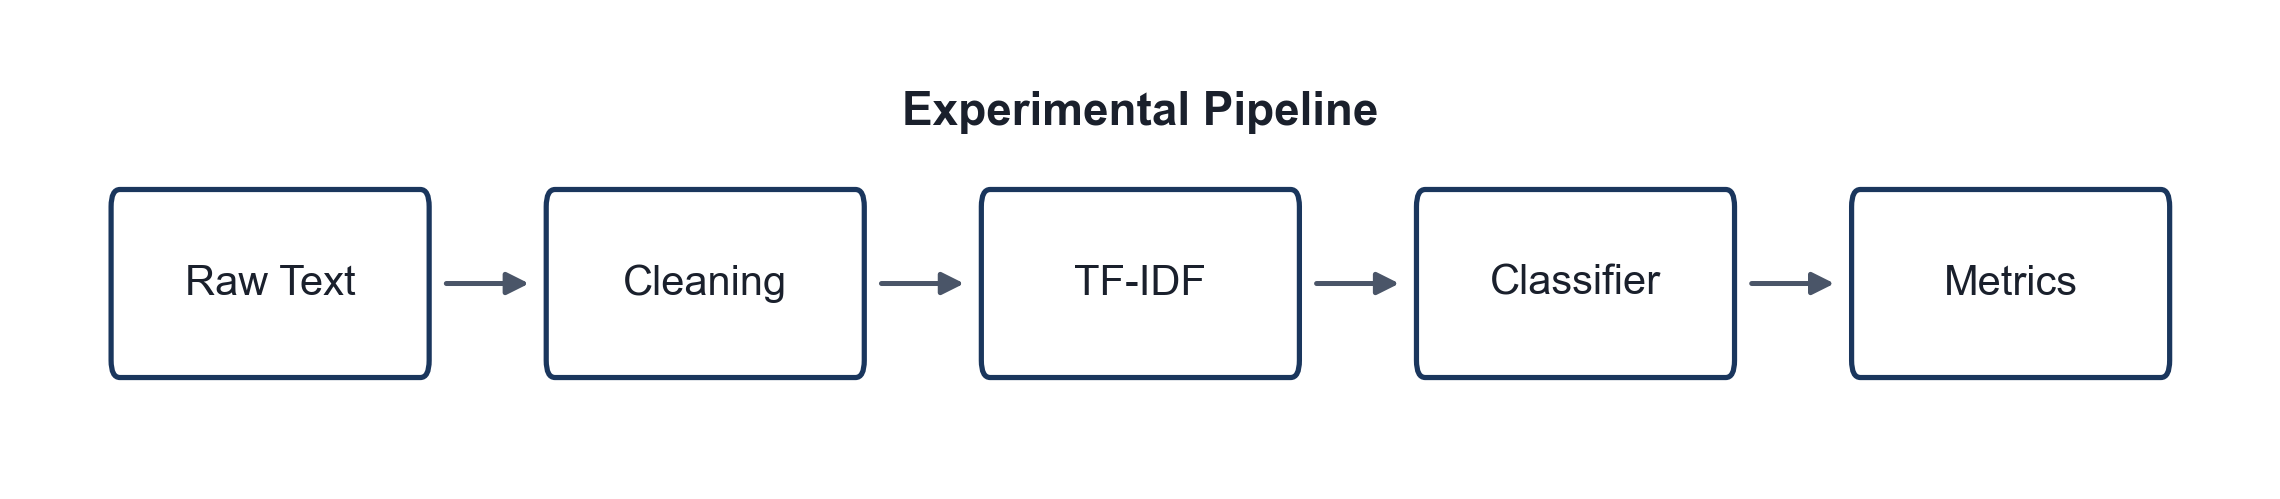
\includegraphics[width=0.92\textwidth]{figures/fig1_pipeline.png}
\caption{End-to-end experimental pipeline. The same preprocessing and vectorization steps are applied before training each classifier to ensure fair comparison.}
\label{fig:pipeline}
\end{figure}

\subsection{Problem formulation}

Let $\mathcal{D}=\{(x_i,y_i)\}_{i=1}^{N}$ denote a labeled corpus, where $x_i$ is a text document and $y_i \in \{1,\ldots,C\}$ is a class label. The goal is to learn a classifier $f_{\theta}:\mathcal{X}\rightarrow\mathcal{Y}$ that maximizes predictive quality while minimizing computational cost during training and inference. We treat model selection as a bi-objective problem:
\begin{equation}
\max_{\theta}\; \mathrm{F1}(f_{\theta}) \quad \text{subject to} \quad T_{\text{train}}(\theta) \le \tau_t,\; T_{\text{infer}}(\theta) \le \tau_i,\; S_{\text{model}}(\theta) \le \tau_s,
\label{eq:objective}
\end{equation}
where $T_{\text{train}}$, $T_{\text{infer}}$, and $S_{\text{model}}$ denote training time, inference latency, and model size, respectively, and $\tau_t$, $\tau_i$, and $\tau_s$ represent deployment budgets.

\subsection{Text preprocessing and feature extraction}

All models share the same preprocessing and vectorization stages:
\begin{enumerate}
    \item Convert text to lowercase.
    \item Remove punctuation, digits, and extra whitespace.
    \item Tokenize documents using whitespace splitting.
    \item Remove English stop words.
    \item Transform tokens into TF-IDF features using scikit-learn's \texttt{TfidfVectorizer}~\cite{pedregosa2011scikit}.
\end{enumerate}

The TF-IDF weight of term $t$ in document $d$ is:
\begin{equation}
\mathrm{TFIDF}(t,d)=\mathrm{TF}(t,d)\cdot \log\!\left(\frac{N}{\mathrm{DF}(t)+1}\right),
\label{eq:tfidf}
\end{equation}
where $N$ is the number of documents and $\mathrm{DF}(t)$ is the document frequency of term $t$.

Using a single shared vectorizer prevents confounding effects caused by inconsistent feature spaces across models.

\subsection{Classifiers}

We evaluate five lightweight classical models frequently used in text mining:
\begin{itemize}
    \item \textbf{Logistic Regression (LR):} Linear probabilistic classifier; a strong baseline for sparse text features.
    \item \textbf{Linear Support Vector Machine (SVM):} Maximum-margin linear classifier; effective for high-dimensional text data~\cite{joachims1998text}.
    \item \textbf{Multinomial Naive Bayes (MNB):} Probabilistic generative model with conditional independence assumptions.
    \item \textbf{Random Forest (RF):} Bagged ensemble of decision trees capturing non-linear interactions.
    \item \textbf{XGBoost (XGB):} Gradient-boosted trees optimized for speed and performance~\cite{chen2016xgboost}.
\end{itemize}

Hyperparameters are listed in Table~\ref{tab:hyperparams}. We use fixed, literature-standard defaults rather than exhaustive tuning. This choice reflects a \emph{resource-constrained deployment scenario} in which large hyperparameter searches may be impractical: extensive grid search would increase training cost and confound efficiency comparisons among models. Accuracy-first production systems may still benefit from additional tuning at higher computational expense; we discuss this trade-off in Section~\ref{sec:discussion}.

\begin{table}[t]
\caption{Classifier hyperparameters}\label{tab:hyperparams}
\begin{tabular}{@{}ll@{}}
\toprule
Model & Configuration \\
\midrule
Logistic Regression & $C=1.0$, \texttt{solver=lbfgs}, \texttt{max\_iter=1000} \\
Linear SVM & $C=1.0$, \texttt{loss=squared\_hinge} \\
Multinomial Naive Bayes & $\alpha=1.0$ \\
Random Forest & \texttt{n\_estimators=100}, \texttt{max\_depth=None} \\
XGBoost & \texttt{n\_estimators=100}, \texttt{max\_depth=6}, \texttt{learning\_rate=0.1} \\
\botrule
\end{tabular}
\end{table}

\subsection{Evaluation metrics}

\subsubsection{Predictive metrics}
We report Accuracy, Precision, Recall, and F1-score. For AG News, macro-averaged scores are used to avoid bias toward majority classes.

\subsubsection{Efficiency metrics}
\begin{itemize}
    \item \textbf{Training time} ($T_{\text{train}}$): wall-clock seconds to fit the model.
    \item \textbf{Inference latency} ($T_{\text{infer}}$): milliseconds required to classify 1{,}000 test documents after model training.
    \item \textbf{Model size} ($S_{\text{model}}$): disk size of the serialized model in megabytes.
\end{itemize}

\subsubsection{Composite efficiency score}
To support visual comparison in Figure~\ref{fig:f1_latency}, we compute a non-standard composite score that is \textbf{not} part of established benchmarking practice:
\begin{equation}
E = \frac{\mathrm{F1}}{\log(1 + T_{\text{infer}})}.
\label{eq:efficiency}
\end{equation}
Unlike standard metrics such as F1-score or wall-clock latency, $E$ is an ad hoc ratio defined for this study only; it has no widely accepted definition in the text-classification literature and should not be treated as a validated deployment criterion. The logarithmic term compresses the scale of inference latency so that large latency values do not dominate visual comparisons, following common log-scaling practice in performance analysis~\cite{wang2024atcbench}. Higher values indicate better accuracy relative to inference cost, but $E$ is reported solely to summarize the accuracy-latency trade-off in tables and figures. It is \emph{not} used for formal model selection or hypothesis testing; raw F1, $T_{\text{train}}$, $T_{\text{infer}}$, and $S_{\text{model}}$ should be prioritized according to domain constraints. Because $E$ is monotonically increasing in F1 and decreasing in $T_{\text{infer}}$, it preserves rank ordering along single dimensions but should not replace multi-criteria deployment decisions.

\section{Experimental setup}\label{sec:setup}

\subsection{Datasets}

Two public English datasets are used to represent distinct text-classification regimes while keeping total CPU runtime manageable:
\begin{itemize}
    \item \textbf{SMS Spam Collection}~\cite{almeida2011sms}: binary classification of SMS messages into \textit{ham} or \textit{spam}. Total samples: 5{,}574. Train/test split: 80/20 with stratification.
    \item \textbf{AG News}~\cite{zhang2015character}: four-class news categorization (\textit{World}, \textit{Sports}, \textit{Business}, \textit{Science/Technology}). The public corpus contains 120{,}000 training and 7{,}600 test documents. To keep the full five-model benchmark reproducible on a 2-core CPU within a few minutes, we draw a stratified random subset of 20{,}000 documents (5{,}000 per class) using seed~42. This preserves the original class balance while reducing vocabulary size and training cost for tree-based models. Prior AG News studies report that linear TF-IDF classifiers remain strong baselines on both full and reduced corpora~\cite{zhang2015character,wang2024atcbench}; subsampling therefore primarily affects absolute runtime and ensemble-model fit rather than the expected ranking of linear methods. We do not claim that subset results transfer numerically to the full 127{,}600-document corpus without re-measurement, but the subset is sufficient for relative model comparison under identical preprocessing within this study. Train/test split: 80/20 with stratification.
\end{itemize}

We acknowledge that two datasets cannot represent all text domains (e.g., sentiment, toxicity, legal, or biomedical text). They were selected to span short binary messages and multi-class news articles under a fixed experimental budget.

Table~\ref{tab:datasets} summarizes dataset properties.

\begin{table}[t]
\caption{Dataset summary}\label{tab:datasets}
\begin{tabular}{@{}lccccc@{}}
\toprule
Dataset & Task & Classes & Total & Train & Test \\
\midrule
SMS Spam & Binary spam detection & 2 & 5{,}574 & 4{,}459 & 1{,}115 \\
AG News & News topic classification & 4 & 20{,}000 & 16{,}000 & 4{,}000 \\
\botrule
\end{tabular}
\end{table}

\subsection{Implementation and reproducibility protocol}

Experiments are implemented in Python~3.12 using scikit-learn, XGBoost, pandas, and NumPy~\cite{pedregosa2011scikit,chen2016xgboost}. Table~\ref{tab:hardware} summarizes the hardware and software environment. No GPU was used.

\begin{table}[t]
\caption{Hardware and software environment}\label{tab:hardware}
\begin{tabular}{@{}ll@{}}
\toprule
Component & Specification \\
\midrule
Processor & Intel Xeon CPU @ 2.20~GHz \\
Cores & 2 \\
System memory & 12~GB RAM \\
Operating system & Ubuntu 22.04 LTS (64-bit) \\
Python & 3.12 \\
Key libraries & scikit-learn, XGBoost, pandas, NumPy \\
\botrule
\end{tabular}
\end{table}

To improve reproducibility:
\begin{itemize}
    \item Random seed fixed to 42 for splitting, vectorization, and model initialization.
    \item Identical TF-IDF settings across all models: max\_features=20{,}000, ngram\_range=(1,2), min\_df=2.
    \item Each experiment repeated 3 times with different stratified splits; mean values, 95\% confidence intervals, and Wilcoxon tests reported.
    \item Models serialized with \texttt{joblib} for size measurement.
\end{itemize}

\subsubsection{Number of repeated runs}

We use three repeated stratified splits rather than five-fold cross-validation. Three runs balance statistical reliability and computational cost: they capture run-to-run variability while keeping the full benchmark reproducible on modest CPU hardware within a few minutes. Additional repetitions would improve statistical power but were not used here to preserve a lightweight evaluation protocol.

\subsection{Experimental protocol}

For each dataset and classifier, the protocol is:
\begin{enumerate}
    \item Split data into training and test sets with stratification.
    \item Fit TF-IDF vectorizer on training text only.
    \item Transform train and test sets.
    \item Train classifier and record $T_{\text{train}}$.
    \item Predict test labels and compute predictive metrics.
    \item Measure $T_{\text{infer}}$ over the full test set and compute $S_{\text{model}}$.
\end{enumerate}

This strict ordering prevents data leakage and ensures timing measurements reflect realistic deployment.

\section{Results}\label{sec:results}

\subsection{Classification performance}

Table~\ref{tab:classification} reports predictive performance on both datasets.

\begin{table}[t]
\caption{Classification performance of lightweight models (mean over 3 repeated runs)}\label{tab:classification}
\begin{tabular*}{\textwidth}{@{\extracolsep\fill}lccccc}
\toprule
Dataset & Model & Accuracy & Precision & Recall & F1-score \\
\midrule
\multirow{5}{*}{SMS Spam}
 & Logistic Regression & 96.8 & 98.0 & 77.4 & 86.5 \\
 & Linear SVM          & 98.5 & 97.1 & 91.3 & 94.1 \\
 & Naive Bayes         & 97.1 & 100.0 & 78.1 & 87.7 \\
 & Random Forest       & 97.9 & 99.7 & 84.8 & 91.6 \\
 & XGBoost             & 97.2 & 97.6 & 81.0 & 88.5 \\
\midrule
\multirow{5}{*}{AG News}
 & Logistic Regression & 90.2 & 90.2 & 90.2 & 90.2 \\
 & Linear SVM          & 90.0 & 90.0 & 90.0 & 90.0 \\
 & Naive Bayes         & 90.0 & 90.0 & 90.0 & 90.0 \\
 & Random Forest       & 85.4 & 85.4 & 85.4 & 85.4 \\
 & XGBoost             & 82.7 & 83.0 & 82.7 & 82.8 \\
\botrule
\end{tabular*}
\end{table}

On SMS Spam, Linear SVM achieves the highest mean F1-score of 94.1\%. On AG News, Logistic Regression obtains the best mean macro F1-score of 90.2\%. Table~\ref{tab:f1_ci} reports 95\% confidence intervals for F1-scores; intervals are wide because only three repeated runs were used, so rankings should be interpreted cautiously. As shown in Section~\ref{sec:stats}, margins among top models are not statistically significant at $\alpha=0.05$. On SMS Spam, Logistic Regression and Naive Bayes achieve high precision (98.0\% and 100.0\%) but lower recall on the minority \textit{spam} class (77.4\% and 78.1\%), whereas Linear SVM balances both (97.1\% precision, 91.3\% recall). For spam-filtering deployments that prioritize catching malicious messages, recall on the positive class may outweigh raw F1; confusion matrices (Figure~\ref{fig:confusion}) provide a clearer basis for selection than a single aggregate score.

\begin{table}[t]
\caption{F1-score with 95\% confidence intervals ($n=3$ runs; $t$-distribution)}\label{tab:f1_ci}
\begin{tabular*}{\textwidth}{@{\extracolsep\fill}lcc}
\toprule
Dataset & Model & F1 (\%) [95\% CI] \\
\midrule
\multirow{5}{*}{SMS Spam}
 & Logistic Regression & 86.5 [83.2, 89.8] \\
 & Linear SVM          & 94.1 [89.2, 99.0] \\
 & Naive Bayes         & 87.7 [85.0, 90.3] \\
 & Random Forest       & 91.6 [88.7, 94.6] \\
 & XGBoost             & 88.5 [83.7, 93.3] \\
\midrule
\multirow{5}{*}{AG News}
 & Logistic Regression & 90.2 [90.1, 90.4] \\
 & Linear SVM          & 90.0 [88.9, 91.0] \\
 & Naive Bayes         & 90.0 [89.2, 90.7] \\
 & Random Forest       & 85.4 [84.0, 86.7] \\
 & XGBoost             & 82.8 [81.4, 84.1] \\
\botrule
\end{tabular*}
\end{table}

\subsection{Efficiency analysis}

Table~\ref{tab:efficiency_sms} and Table~\ref{tab:efficiency_ag} report efficiency metrics by dataset. The composite score $E$ (Equation~\ref{eq:efficiency}) is included for visualization only and should be interpreted alongside the primary metrics $T_{\text{train}}$, $T_{\text{infer}}$, and $S_{\text{model}}$.

\begin{table}[t]
\caption{Efficiency metrics on SMS Spam}\label{tab:efficiency_sms}
\begin{tabular*}{\textwidth}{@{\extracolsep\fill}lcccc}
\toprule
Model & $T_{\text{train}}$ (s) & $T_{\text{infer}}$ (ms/1k) & Size (MB) & $E$ \\
\midrule
Logistic Regression & 0.2 & 0.03 & 0.30 & 26.78 \\
Linear SVM          & 0.2 & 0.02 & 0.30 & 49.66 \\
Naive Bayes         & 0.2 & 0.03 & 0.46 & 26.62 \\
Random Forest       & 1.9 & 0.07 & 5.81 & 12.90 \\
XGBoost             & 1.6 & 0.04 & 0.38 & 27.09 \\
\botrule
\end{tabular*}
\end{table}

\begin{table}[t]
\caption{Efficiency metrics on AG News}\label{tab:efficiency_ag}
\begin{tabular*}{\textwidth}{@{\extracolsep\fill}lcccc}
\toprule
Model & $T_{\text{train}}$ (s) & $T_{\text{infer}}$ (ms/1k) & Size (MB) & $E$ \\
\midrule
Logistic Regression & 5.6 & 0.06 & 1.36 & 14.40 \\
Linear SVM          & 2.3 & 0.06 & 1.36 & 16.23 \\
Naive Bayes         & 1.9 & 0.05 & 1.97 & 19.67 \\
Random Forest       & 29.7 & 0.10 & 84.84 & 8.70 \\
XGBoost             & 114.0 & 0.07 & 1.60 & 11.94 \\
\botrule
\end{tabular*}
\end{table}

Linear SVM achieves the lowest mean inference latency on SMS Spam (0.02~ms per 1{,}000 samples), whereas Random Forest and XGBoost incur substantially higher training cost on AG News (114~s for XGBoost versus 2.3~s for Linear SVM). Summed over all five models and both datasets, the benchmark requires approximately 2.6 minutes of CPU training time per repetition (157~s mean wall-clock), making the protocol suitable for classroom reproduction and rapid prototyping. The accuracy-efficiency trade-off is most visible on AG News due to its larger vocabulary and higher class count.

\subsection{Visual analysis}

Figure~\ref{fig:f1_latency} visualizes the relationship between F1-score and inference latency. Figure~\ref{fig:confusion} shows confusion matrices for the best model on each dataset. Figure~\ref{fig:training_time} compares training time across models.

\begin{figure}[t]
\centering
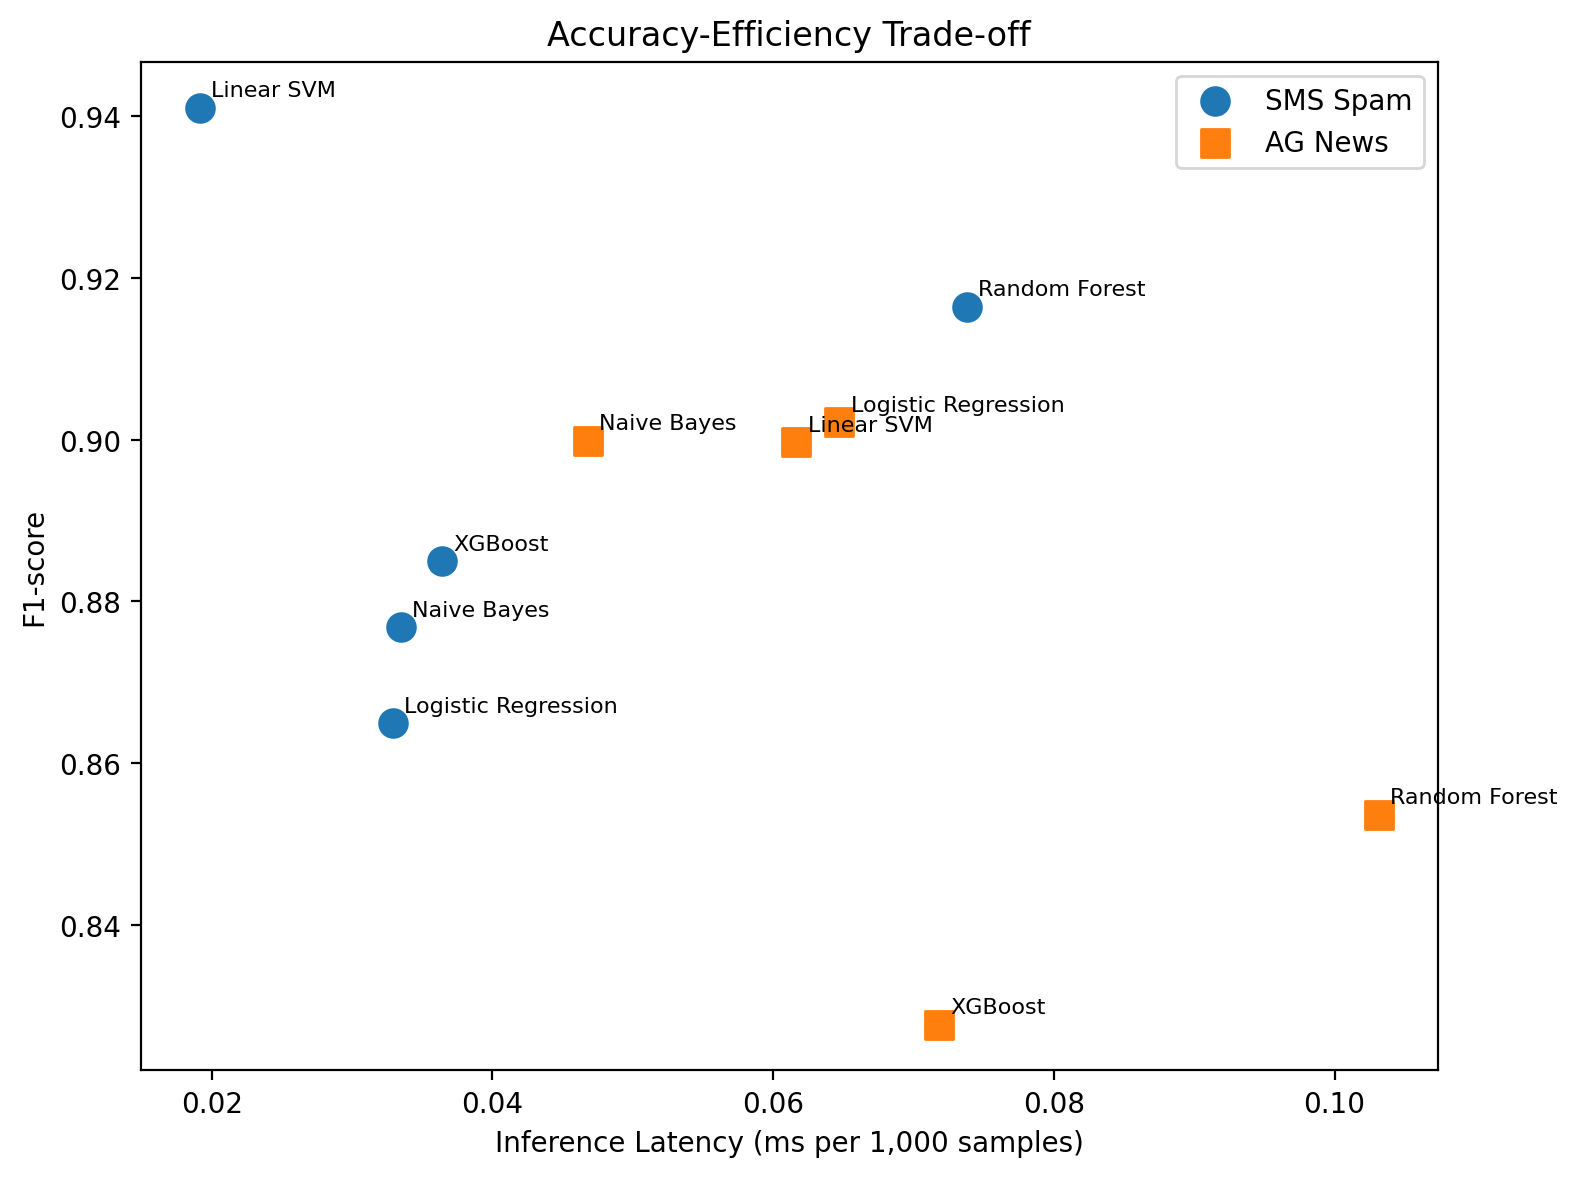
\includegraphics[width=0.92\textwidth]{figures/fig2_f1_latency.png}
\caption{Accuracy-efficiency trade-off for all classifiers. Points closer to the upper-left region indicate higher F1 with lower latency.}
\label{fig:f1_latency}
\end{figure}

\begin{figure}[t]
\centering
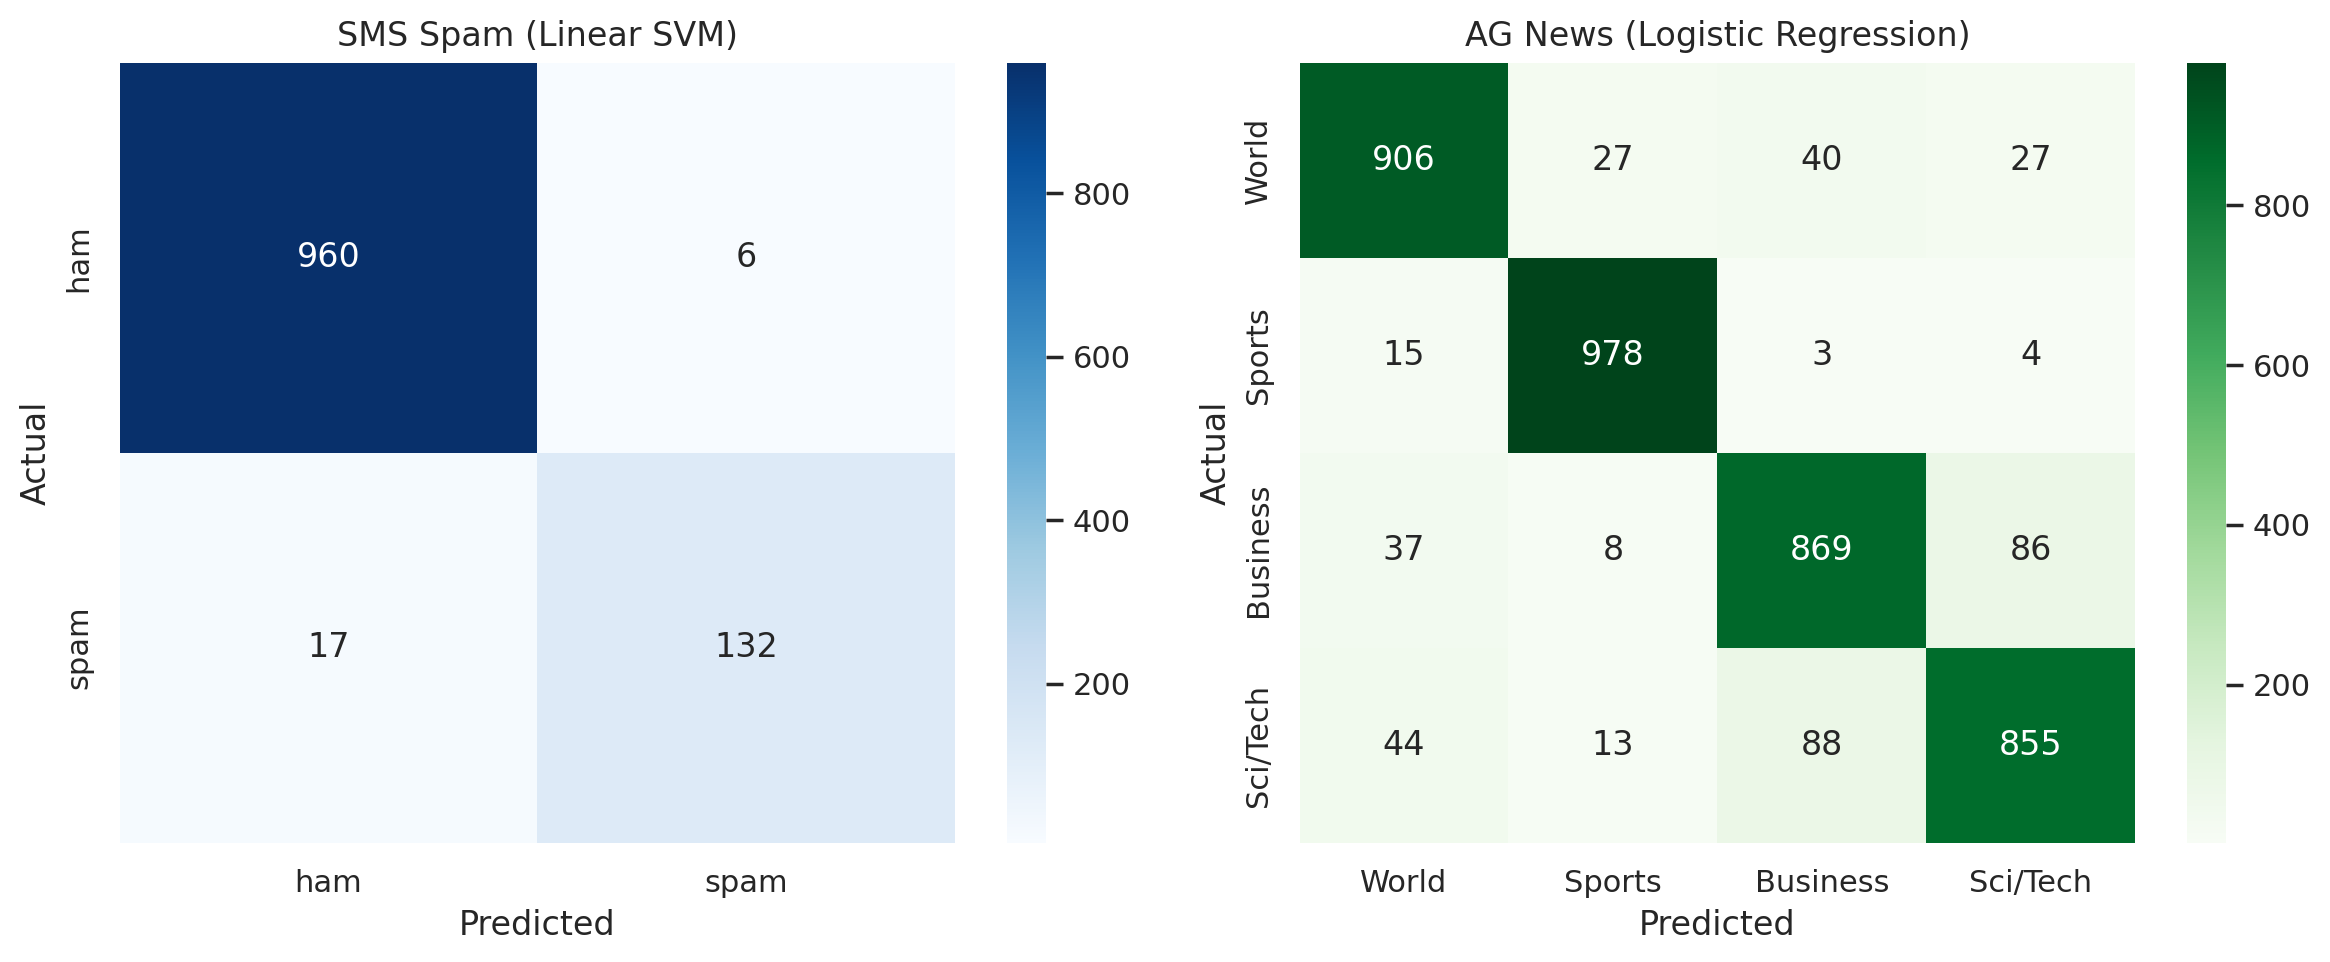
\includegraphics[width=0.92\textwidth]{figures/fig3_confusion.png}
\caption{Confusion matrices for the best-performing model on each dataset (Linear SVM on SMS Spam; Logistic Regression on AG News).}
\label{fig:confusion}
\end{figure}

\begin{figure}[t]
\centering
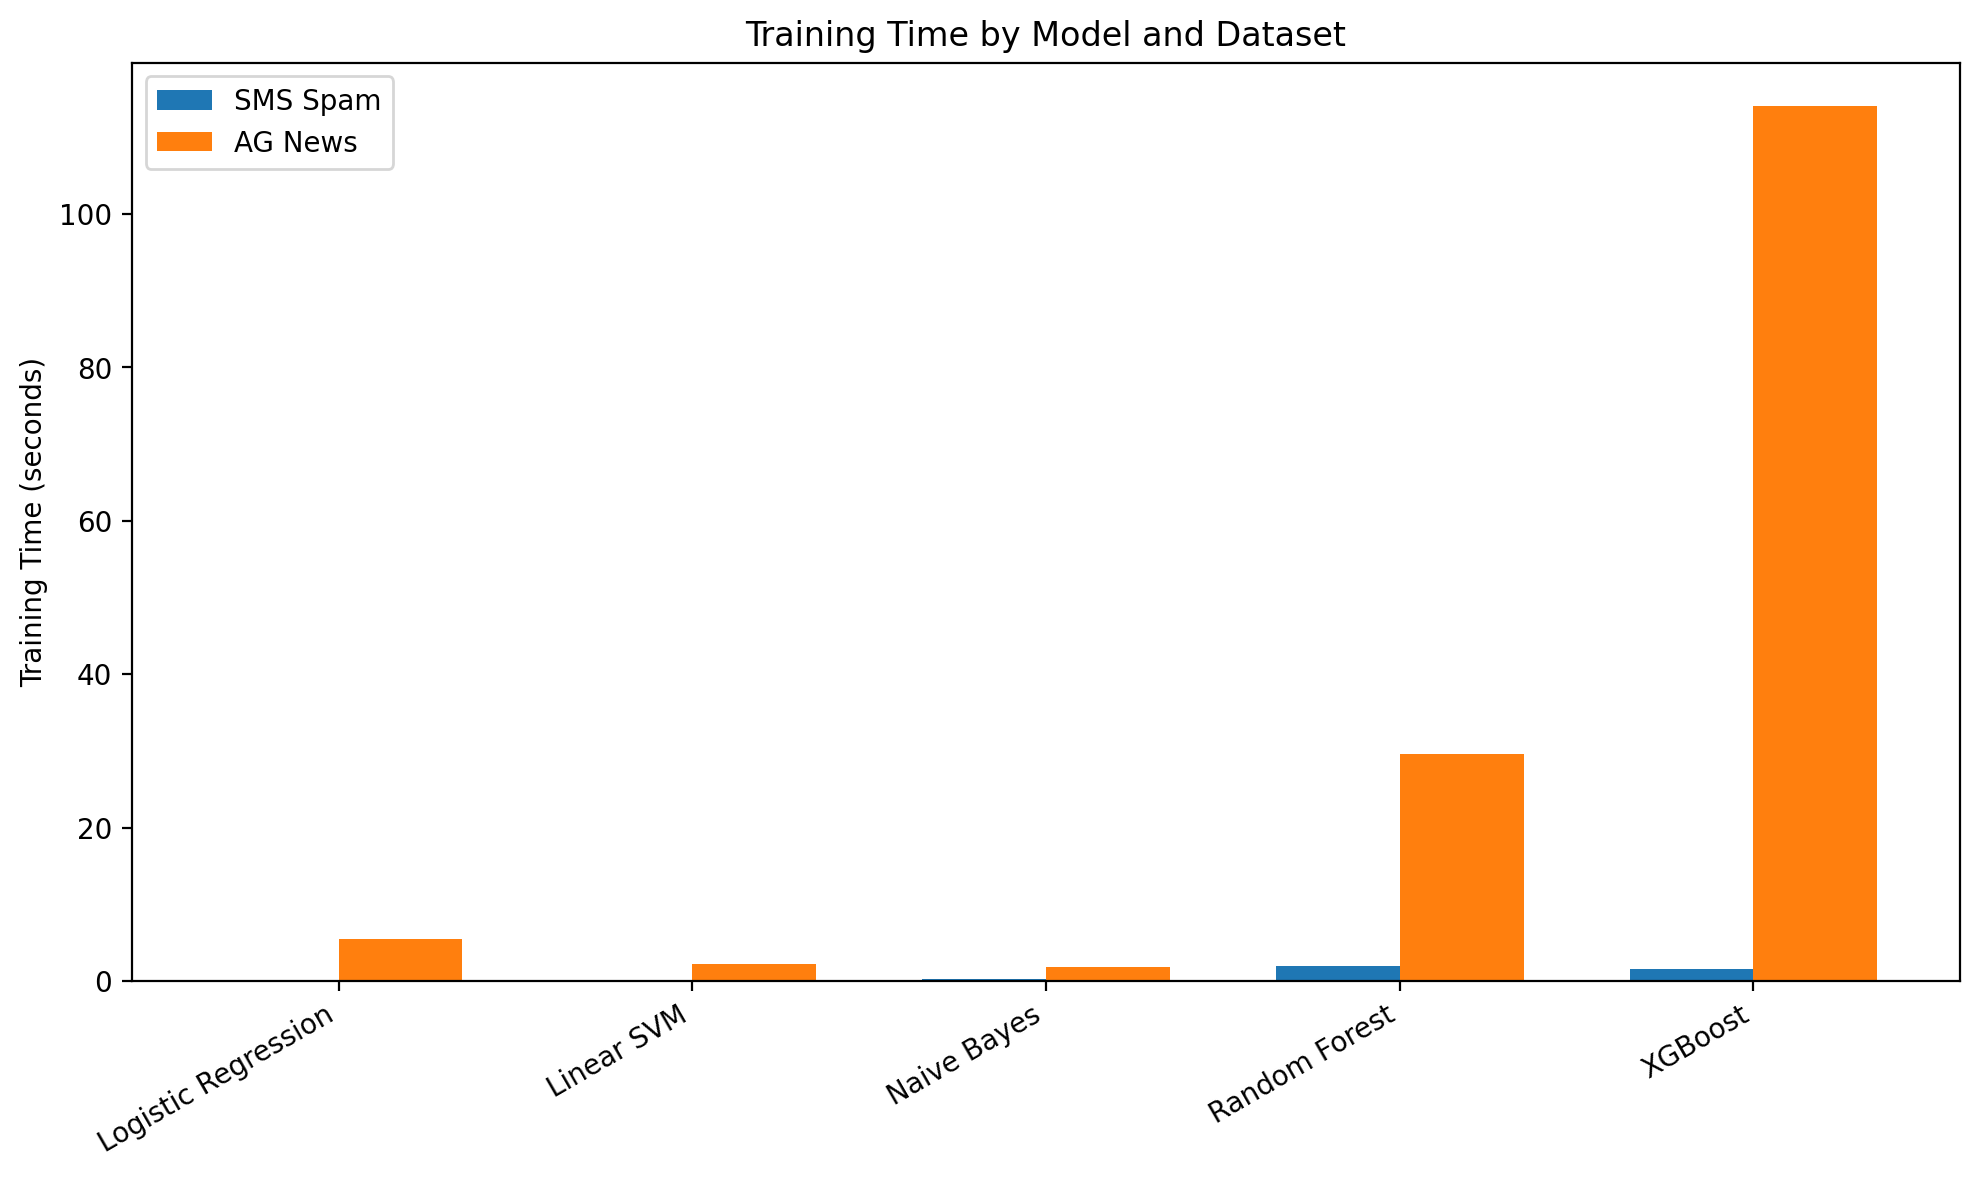
\includegraphics[width=0.92\textwidth]{figures/fig4_training_time.png}
\caption{Training time comparison across models and datasets.}
\label{fig:training_time}
\end{figure}

\subsection{Model selection summary}

Table~\ref{tab:guidelines} translates empirical findings into practical recommendations.

\begin{table}[t]
\caption{Practical model-selection guidelines derived from the benchmark}\label{tab:guidelines}
\begin{tabular}{@{}p{3.1cm}p{4.1cm}p{6.3cm}@{}}
\toprule
Priority & Recommended model & Rationale \\
\midrule
Highest F1 on SMS Spam & Linear SVM & Best F1 (94.1\%) with balanced spam recall (91.3\%) \\
Highest F1 on AG News & Logistic Regression & Best macro F1 (90.2\%) among all models \\
Lowest latency & Linear SVM & 0.02~ms per 1{,}000 samples on SMS Spam \\
Smallest model size & Linear SVM / LR & 0.30~MB serialized pipeline on SMS Spam \\
Best overall trade-off & Linear SVM & Highest SMS F1 with lowest latency; $E=49.66$ (not used for selection) \\
Spam recall priority & Linear SVM & 91.3\% spam recall vs.\ 77.4\% (LR) and 78.1\% (MNB) \\
\botrule
\end{tabular}
\end{table}

\subsection{Statistical significance analysis}\label{sec:stats}

Because each model was evaluated over three repeated stratified splits, we apply the Wilcoxon signed-rank test to paired F1-scores for the top two models on each dataset. Table~\ref{tab:stats} reports the results. Neither comparison reaches conventional significance at $\alpha=0.05$, so small mean F1 differences (e.g., 90.2\% versus 90.0\% on AG News) should not be over-interpreted without additional runs or larger test sets.

\begin{table}[t]
\caption{Wilcoxon signed-rank tests on F1-scores ($n=3$ runs per model)}\label{tab:stats}
\begin{tabular}{@{}llcc@{}}
\toprule
Dataset & Comparison & $p$-value & Significant ($\alpha=0.05$) \\
\midrule
SMS Spam & Linear SVM vs.\ Random Forest & 0.25 & No \\
AG News & Logistic Regression vs.\ Linear SVM & 0.50 & No \\
\botrule
\end{tabular}
\end{table}

With only three paired runs, Wilcoxon $p$-values are coarse and statistical power is limited (Table~\ref{tab:f1_ci}). Non-significant results do not establish model equivalence; they indicate only that the available sample is too small for stronger inference. These tests are reported as supplementary summaries of run-to-run variability rather than as confirmatory evidence.

\section{Discussion}\label{sec:discussion}

\subsection{Interpretation of results}

Linear models (Logistic Regression and Linear SVM) consistently deliver the strongest predictive performance on TF-IDF features in this study. This aligns with decades of text-classification research showing that sparse high-dimensional representations pair naturally with linear decision boundaries~\cite{joachims1998text,sebastiani2002machine}. Tree ensembles underperform on AG News, likely because sparse TF-IDF vectors provide limited benefit from axis-aligned splits without extensive tuning, while remaining competitive on SMS Spam.

On SMS Spam, the minority \textit{spam} class drives metric differences among top models. Linear SVM improves spam recall relative to Logistic Regression and Naive Bayes without sacrificing precision, which explains its F1 advantage in imbalanced binary filtering. For deployments where false negatives (missed spam) carry higher cost than false positives, recall on the positive class should be weighted explicitly in model selection rather than inferred from accuracy alone.

The highest-accuracy model is not necessarily the most computationally efficient. Linear SVM offers the best balance of SMS Spam F1 and inference speed, whereas XGBoost on AG News requires 114~s of CPU training yet yields the lowest F1 among the five models under default hyperparameters.

\subsection{Comparison with neural baselines}\label{sec:neural}

Neural models were excluded because the study focuses exclusively on classical TF-IDF-based classifiers under CPU-only conditions. Every model in the benchmark consumes the same sparse TF-IDF matrix within a scikit-learn pipeline. Introducing DistilBERT, MiniLM, or FastText would require a separate tokenization and embedding pipeline (PyTorch/TensorFlow, subword vocabularies, and typically GPU acceleration for practical fine-tuning), which falls outside the scope of this comparison. For example, DistilBERT fine-tuning on AG News commonly requires hundreds of megabytes of model weights and GPU-oriented runtimes orders of magnitude above our 2.6-minute classical benchmark~\cite{sanh2020distilbert,wang2024atcbench}; running it on CPU would dominate wall-clock time and shift the study from lightweight deployment guidance to neural-system benchmarking.

We therefore compare against published neural results rather than re-implementing them under a different hardware budget. Table~\ref{tab:literature} summarizes representative AG News results from prior work alongside our classical benchmark; direct numeric comparison is approximate because corpus size, splits, and metrics differ across studies.

\begin{table}[t]
\caption{Representative AG News results from prior work compared with this study (approximate; metrics and data splits differ across sources)}\label{tab:literature}
\begin{tabular}{@{}p{2.8cm}p{3.2cm}cp{3.5cm}@{}}
\toprule
Study & Method & Reported score & Notes \\
\midrule
This work & LR + TF-IDF & 90.2\% macro F1 & 20{,}000-doc stratified subset; CPU \\
Zhang et al.~\cite{zhang2015character} & Character CNN & 91.5\% accuracy & Full 127{,}600-doc corpus; GPU training \\
Wang et al.~\cite{wang2024atcbench} & Classical / LLM suite & F1 varies by model & 22-dataset benchmark; classical models orders of magnitude faster \\
Devlin et al.~\cite{devlin2019bert} & BERT fine-tuning & Typically $>$93\% accuracy & Full-corpus fine-tuning in follow-on work; GPU \\
\botrule
\end{tabular}
\end{table}

Character- and word-level convolutional networks on AG News achieve competitive or higher accuracy but require GPU-oriented training stacks and longer experimentation cycles~\cite{zhang2015character,devlin2019bert}. Wang et al.~\cite{wang2024atcbench} report across 22 datasets that classical models remain orders of magnitude faster than large language models despite lower peak accuracy. Our complete classical benchmark finishes in approximately 2.6 minutes on CPU-only hardware, supporting the use of TF-IDF pipelines for teaching, prototyping, and low-budget deployment when peak accuracy is not the sole objective. A fair experimental neural baseline (e.g., DistilBERT fine-tuned under a fixed GPU time cap with matched train/test splits) is left for future work.

\subsection{Threats to validity}\label{sec:limitations}

This study has several limitations:
\begin{itemize}
    \item \textbf{Scope.} Only two English datasets are evaluated; conclusions may not generalize to sentiment, toxicity, legal, or biomedical domains.
    \item \textbf{Neural baselines.} No transformer or embedding-based model was trained; see Section~\ref{sec:neural} for scope rationale.
    \item \textbf{AG News subsampling.} Results obtained from the 20{,}000-document subset may differ from those of the full corpus; rankings reported here apply to the subset studied.
    \item \textbf{Features.} TF-IDF bag-of-words features do not capture word order or context; contextual embeddings may alter model rankings.
    \item \textbf{Hyperparameters.} Fixed defaults may disadvantage tree-based models relative to an exhaustive search budget.
    \item \textbf{Statistical power.} Three repeated runs yield wide 95\% confidence intervals (Table~\ref{tab:f1_ci}) and limit the sensitivity of significance tests; rankings should be interpreted cautiously.
    \item \textbf{Hardware.} Latency measurements are valid for comparative analysis within this study but may differ on other CPU configurations.
\end{itemize}

\subsection{Applicability to multilingual text}\label{sec:multilingual}

All experiments use English corpora with English stop-word removal. Multilingual deployment introduces vocabulary growth, script-specific tokenization, and class imbalance across languages that our protocol does not evaluate. The classical models studied here remain common baselines in multilingual routing because TF-IDF and linear classifiers scale to language-specific vocabularies without joint multilingual pretraining~\cite{pissinou2025edge,wang2024atcbench}. Character $n$-grams, language-aware stop-word lists, or one-versus-rest training per language can extend the same sklearn pipeline to non-English text with modest code changes, although relative model rankings may shift when morphology is rich or labeled data are imbalanced across locales. Our English-only results should therefore be viewed as a starting point for multilingual extensions rather than as language-independent conclusions. Extending the benchmark to multilingual corpora such as FLORES or language-balanced news sets is a logical direction for future work.

\section{Conclusion}\label{sec:conclusion}

We presented a comparative study of five classical lightweight machine learning models for text classification under CPU-only constraints. Using a unified TF-IDF pipeline on SMS Spam and AG News, we evaluated both predictive quality and deployment cost. Linear SVM and Logistic Regression achieved the best mean F1-scores, while Linear SVM also delivered the lowest inference latency and the strongest spam recall on the imbalanced SMS corpus. Statistical tests and confidence intervals indicate that differences among top models are not statistically significant at $\alpha=0.05$ with three runs. These findings are specific to TF-IDF-based classical machine-learning pipelines and should not be extrapolated to contextual-embedding or neural architectures without further evaluation.

Future work will: (1)~extend the benchmark to additional domains such as sentiment and toxicity detection; (2)~include multilingual datasets and domain-adaptation settings to test whether linear-model advantages persist across languages; (3)~include a compact neural baseline (e.g., DistilBERT) under a fixed GPU time budget for direct accuracy comparison; (4)~apply lightweight hyperparameter search to assess whether tree ensembles close the gap with linear models; (5)~report memory-constrained inference benchmarks (e.g., peak RAM under batch-1 serving); and (6)~evaluate streaming and imbalanced data settings relevant to production spam filtering.

\section*{Declarations}

\subsection*{Funding}
Not applicable.

\subsection*{Conflict of interest}
The authors declare no competing interests.

\subsection*{Ethics approval and consent to participate}
Not applicable.

\subsection*{Consent for publication}
Not applicable.

\subsection*{Data availability}
The SMS Spam Collection is available from the UCI Machine Learning Repository (\url{https://archive.ics.uci.edu/dataset/228/sms+spam+collection}). AG News is available from the HuggingFace dataset mirror \url{https://huggingface.co/datasets/sh0416/ag_news}.

\subsection*{Code availability}
Experiment code, configuration files, and result CSVs are publicly available at \url{https://github.com/ChaituMokkapati/lightweight-ml-text-classification}. A version-tagged archival release is deposited on Zenodo at \url{https://doi.org/10.5281/zenodo.20781407} (DOI: \texttt{10.5281/zenodo.20781407}).

\subsection*{Author contribution}
Chaitanya Mokkapati: conceptualization, methodology, software, validation, visualization, writing, original draft. Dr.\ Prasad Devarasetty: supervision, writing, review and editing. Nagulmeera Syyed: investigation, writing, review and editing.

\bibliography{references}

\end{document}
